\section{بررسی عملکرد فیلتر \lr{Anti-aliasing} پیشرفته (۹ درایه‌ای)}

در این مرحله، قصد داریم از یک فیلتر پایین‌گذر بزرگ‌تر و قوی‌تر استفاده کنیم. فیلتر قبلی تنها ۳ درایه داشت، اما در این بخش از یک فیلتر ۹ درایه‌ای استفاده می‌کنیم که تقریب بسیار بهتری از یک فیلتر گوسی (Gaussian) پهن است. هدف این است که ببینیم اعمال یک فیلتر قوی‌تر چه تأثیری روی مهار الیاسینگ و همچنین کیفیت بصری تصویر (میزان تاری) می‌گذارد.

\subsection*{۱. تعریف فیلتر پیشرفته}
ابتدا آرایه‌ی مربوط به فیلتر جدید را تعریف می‌کنیم:

\begin{codebox}[\lr{Advanced Low-pass Filter}]
\begin{lstlisting}[language=Python]
    # تعریف فیلتر ۹ درایه‌ای
    kernel_1d_new = np.array([0.0267, 0.0169, 0.0782, 0.2669, 0.6029, 
                              0.2669, 0.0782, 0.0169, 0.0267])
\end{lstlisting}
\end{codebox}

همان‌طور که از مقادیر پیداست، بیشترین وزن (۰.۶۰۲۹) به پیکسل مرکزی اختصاص دارد و وزن‌ها با الگویی زنگوله‌ای (شبیه به توزیع نرمال) به سمت لبه‌ها کاهش می‌یابند. پهن‌تر بودن این فیلتر به معنای میانگین‌گیری از همسایگی بزرگ‌تر است که منجر به حذف شدیدتر فرکانس‌های بالا (لبه‌های تیز) می‌شود.

\subsection*{۲. اعمال فیلتر قوی و کاهش ابعاد (نرخ ۴)}
عملیات را با اعمال فیلتر جدید آغاز می‌کنیم:

\begin{codebox}[\lr{Filtering and Downsampling - Rate 4}]
\begin{lstlisting}[language=Python]
    # اعمال فیلتر ۹ درایه‌ای در دو راستا
    filtered_img_new = cv2.sepFilter2D(img, -1, kernel_1d_new, kernel_1d_new)
    
    # کوچک‌سازی با نرخ ۴
    down4_img_new = filtered_img_new[::4, ::4]
\end{lstlisting}
\end{codebox}

دستور \lr{\texttt{cv2.sepFilter2D}} این فیلتر سنگین را روی تصویر اعمال می‌کند. به دلیل طولانی‌تر بودن فیلتر، تصویر خروجی (\lr{filtered\_img\_new}) پیش از کوچک شدن، بسیار تارتر از مرحله‌ی قبل خواهد شد تا هیچ فرکانس بالایی نتواند از حد نایکوئیست عبور کند.

\subsection*{۳. پردازش آبشاری برای نرخ ۱۶}
برای رسیدن به نرخ ۱۶، مجدداً از رویکرد آبشاری استفاده می‌کنیم:

\begin{codebox}[\lr{Cascaded Processing - Rate 16}]
\begin{lstlisting}[language=Python]
    # اعمال مجدد فیلتر سنگین روی خروجی نرخ ۴
    filtered_down4_new = cv2.sepFilter2D(down4_img_new, -1, kernel_1d_new, kernel_1d_new)
    
    # کاهش ابعاد نهایی برای نرخ ۱۶
    down16_img_new = filtered_down4_new[::4, ::4]
\end{lstlisting}
\end{codebox}

نکته‌ی بسیار مهم در این قطعه کد این است که تصویرِ نرخ ۴ (که خود به شدت مات شده بود)، **دوباره** تحت تأثیر این فیلتر قوی قرار می‌گیرد. این دو بار فیلتر شدن متوالی، باعث سرکوب کامل هرگونه جزئیات ساختاری در تصویر می‌شود.

\subsection*{نمایش خروجی‌ها (تصویر \lr{Grid})}
در شکل زیر، نتایج بازسازی تصویر \lr{Grid} پس از اعمال این فیلتر قوی نمایش داده شده است. نام‌گذاری فایل‌ها دقیقاً منطبق بر خروجی‌های به‌دست‌آمده است:

\begin{figure}[h!]
    \centering
    \begin{subfigure}{0.48\textwidth}
        \centering
        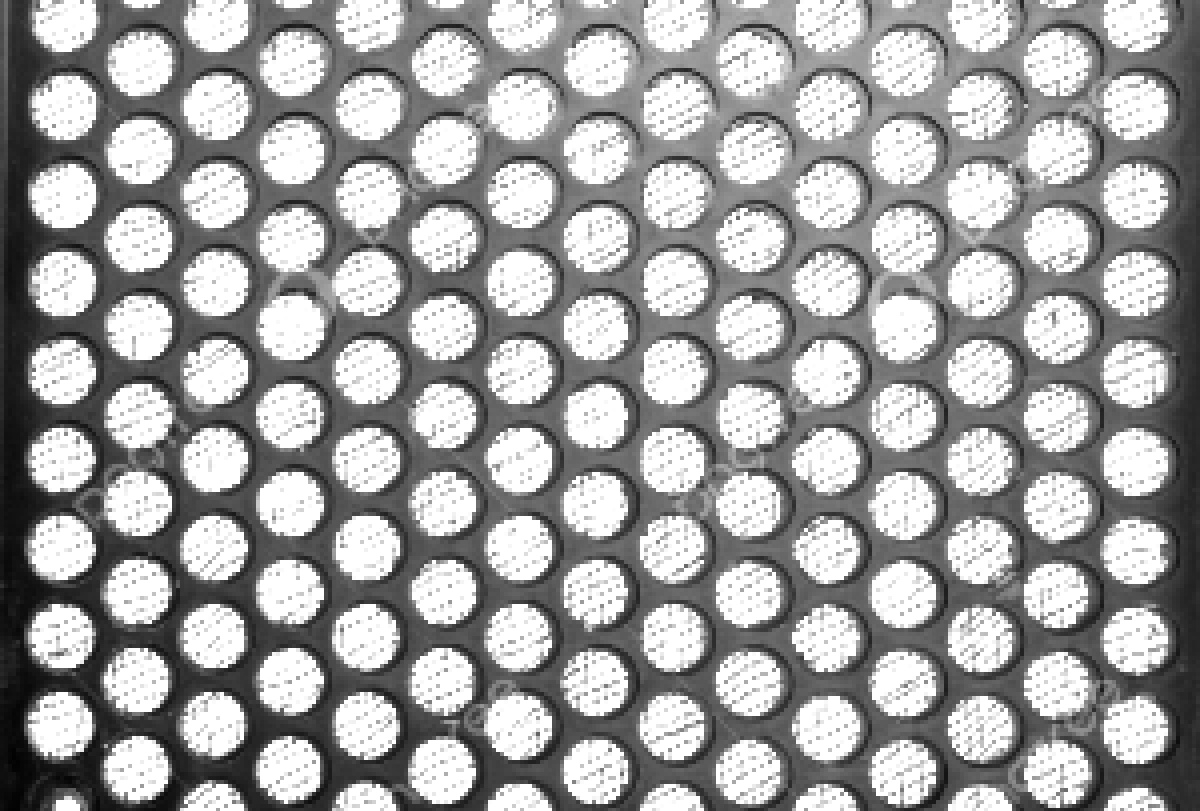
\includegraphics[width=\textwidth]{images/2_Rate4_Nearest_2.jpg}
        \caption{نرخ ۴ - درونیابی نزدیک‌ترین همسایه}
    \end{subfigure}
    \hfill
    \begin{subfigure}{0.48\textwidth}
        \centering
        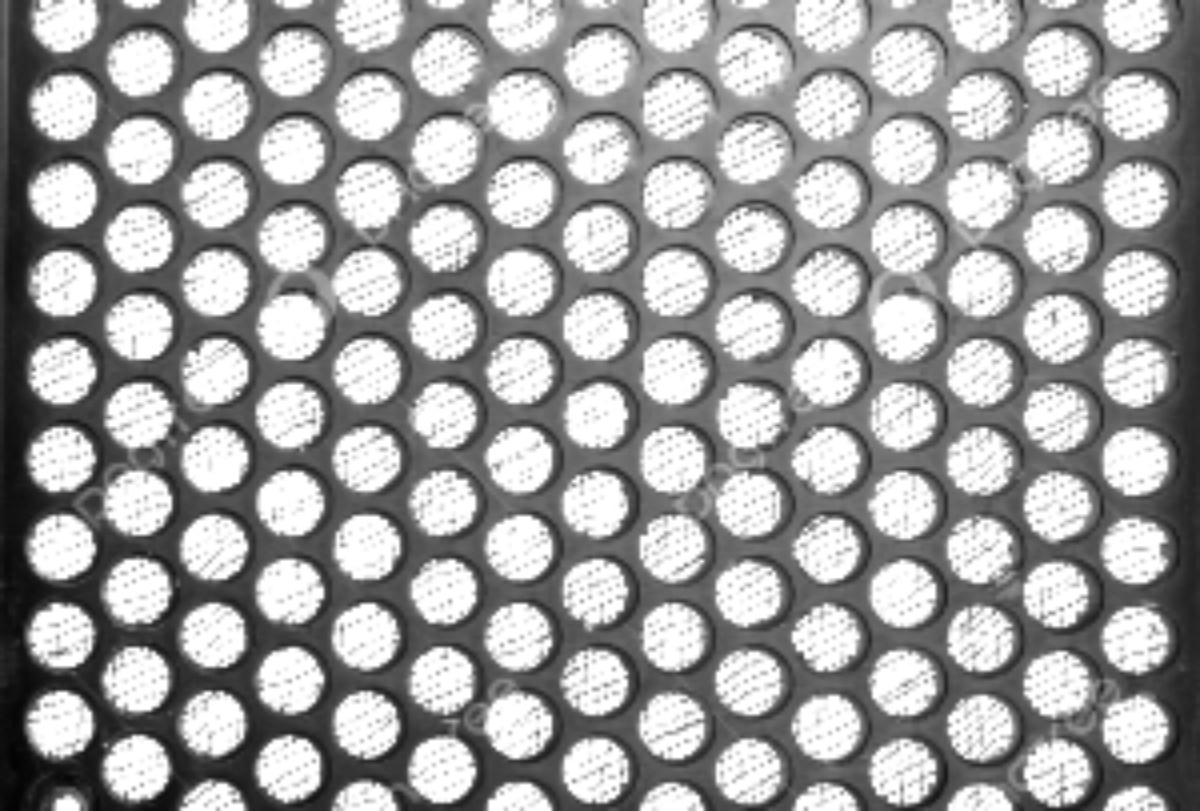
\includegraphics[width=\textwidth]{images/2_Rate4_Bilinear_2.jpg}
        \caption{نرخ ۴ - درونیابی دوخطی}
    \end{subfigure}
    
    \vspace{0.4cm}
    
    \begin{subfigure}{0.48\textwidth}
        \centering
        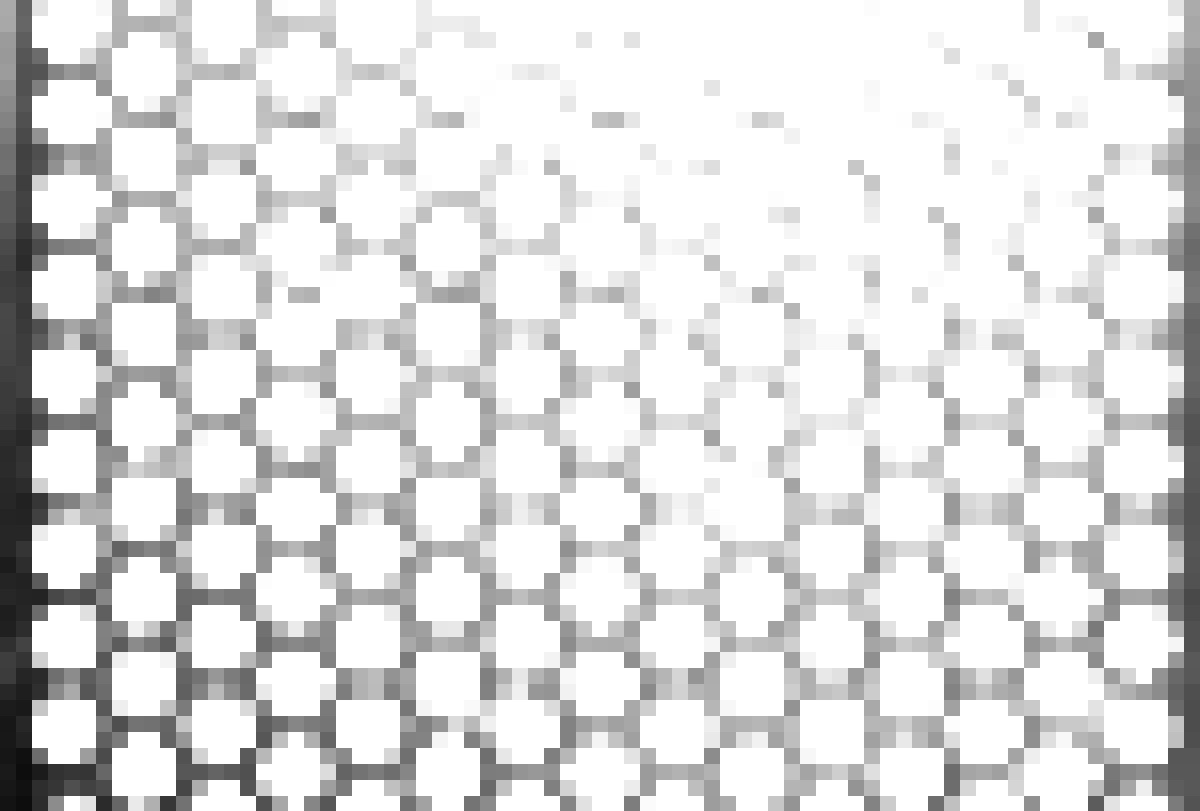
\includegraphics[width=\textwidth]{images/2_Rate16_Nearest_2.jpg}
        \caption{نرخ ۱۶ - درونیابی نزدیک‌ترین همسایه}
    \end{subfigure}
    \hfill
    \begin{subfigure}{0.48\textwidth}
        \centering
        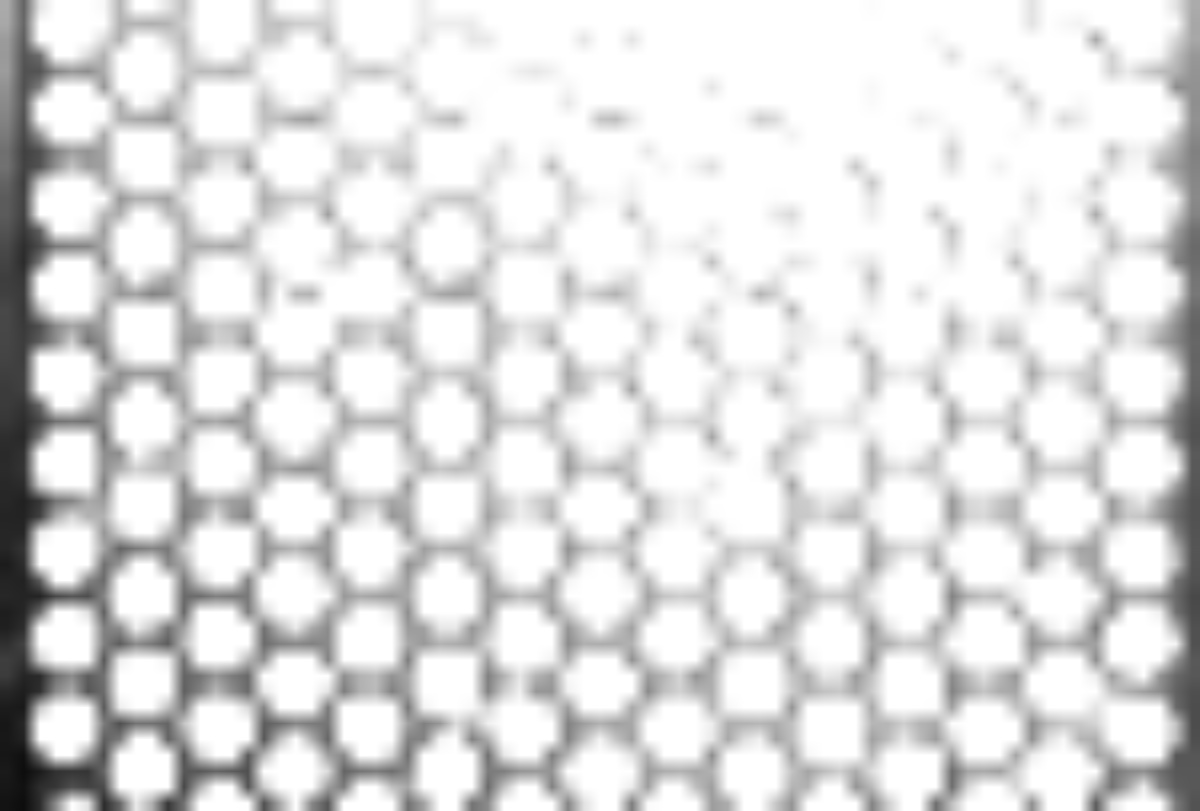
\includegraphics[width=\textwidth]{images/2_Rate16_Bilinear_2.jpg}
        \caption{نرخ ۱۶ - درونیابی دوخطی}
    \end{subfigure}
    \caption{تأثیر اعمال فیلتر پیشرفته (۹ درایه‌ای) بر مهار الیاسینگ و میزان تاری تصویر}
    \label{fig:part4_grid_comparison}
\end{figure}

\subsection*{تحلیل عمیق خروجی‌ها (\lr{Trade-off} بین الیاسینگ و تاری)}
با مشاهده‌ی تصاویر شکل \ref{fig:part4_grid_comparison}، متوجه تغییرات بسیار بنیادین نسبت به مراحل قبل می‌شویم:

\begin{itemize}
    \item \textbf{در نرخ ۴ (حذف کامل \lr{Moiré}):} در این خروجی‌ها، برخلاف بخش‌های قبل، کوچک‌ترین اثری از الگوهای کاذب و مورب (الیاسینگ) دیده نمی‌شود. فیلتر ۹ درایه‌ای موفق شده است تمامی فرکانس‌های خطرساز را حذف کند. با این حال، بهای این موفقیت، تار شدن چشم‌گیر تصویر است؛ لبه‌های دایره‌های شبکه دیگر تیز نیستند و هاله‌ای مات در اطراف آن‌ها شکل گرفته است.
    
    \item \textbf{در نرخ ۱۶ (از بین رفتن سیگنال اصلی):} خروجی‌های نرخ ۱۶ بسیار عجیب به نظر می‌رسند؛ تصویر به شدت محو شده و ساختار شبکه‌ای تقریباً ناپدید شده است. دلیل ریاضی این پدیده آن است که فیلتر ۹ درایه‌ای \textbf{دو بار به صورت متوالی} روی تصویر اعمال شده است. این فیلترینگ مضاعف، تمام انرژی فرکانس‌های بالا و میانی را بلعیده و تنها مؤلفه‌ی \lr{DC} (میانگین روشنایی پیکسل‌ها) و فرکانس‌های بسیار پایین را باقی گذاشته است.
    
    \item \textbf{نتیجه‌گیری علمی:} این مرحله یک درس مهم در پردازش تصویر به همراه دارد: مهار کامل الیاسینگ همیشه به معنای داشتن یک تصویر باکیفیت نیست. فیلتر پایین‌گذر باید با دقت و متناسب با نرخ \lr{Downsampling} انتخاب شود. استفاده از فیلتر بیش از حد قوی (مثل این فیلتر ۹ درایه‌ای برای این تصویر)، اگرچه الیاسینگ را کاملاً نابود می‌کند، اما خودِ سیگنال مفید را نیز از بین برده و اصطلاحاً تصویر را \lr{Over-blur} می‌کند.
\end{itemize}